% Notes content
\part{Condensed Matter}
\chapter{Basic Models of Metals}

\section{The Drude Model}


\begin{figure}[htbp]
  \centering
  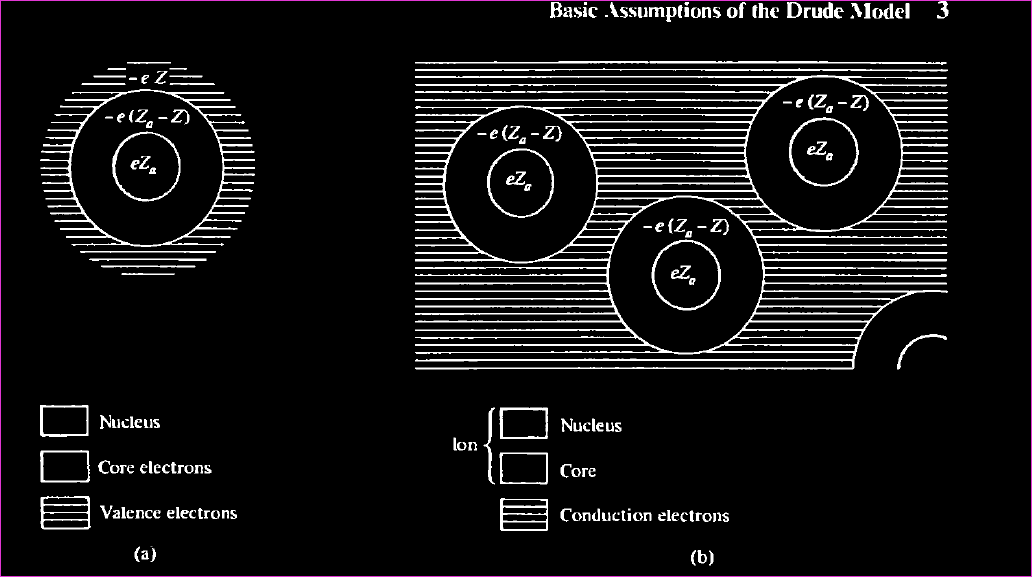
\includegraphics[width=\linewidth]{images/basic_assumptions.png}
\end{figure}

The Drude model assumes that we have immovable nucleus with most extern electons free. A nucleus of some element, has $Z$ protons, and subsequently $Z$ electrons with total charge $-eZ$. 

Let's try to derive somethings. We know that electrical force $\vec{F} = -e\vec{E}$ and $\vec{F} = m\vec{a}$. Thus we have:

\begin{equation}
  \vec{a} = \frac{-eE}{m}
\end{equation}

After a collision, the electron accelerates for a time $t$, gaining velocity:

\begin{equation}
  \Delta{\vec{v}} = \vec{a}\cdot t = \frac{-eEt}{m}
\end{equation}

So the final velocity is:

\begin{equation}
  \vec{v}(t) = \vec{v_0}(t) + \Delta{\vec{v}}
\end{equation}

Well, we assume that the collision randomize \textbf{$\vec{v_0}$} (it's isotropic), its \textbf{average is zero}:

$$
  \langle\vec{v_0}\rangle = 0 \implies \langle\vec{v}(t)\rangle = \frac{-eE\langle t \rangle}{m} $$

We know that $\textbf{j} = -ne\textbf{v}$, so we have:

\begin{equation}
  \textbf{j} = -nev_{avg} = -ne\left(\frac{-eE\tau}{m}\right) = \left(\frac{ne²\tau}{m}\right)E
\end{equation}

Let's define the \textbf{conductivity} ($\sigma$) that tell us how easily a material allows electric charges to move when you apply an electric field (that's created when you make a differential in potential). Then:

\begin{equation}
  \textbf{j} = \sigma \textbf{E}
\end{equation}

Notice that conductivity is the inverse of resistivity:

\begin{equation}
  \sigma = \frac{1}{\rho}
\end{equation}

We can determine the relaxation time $\tau$ usgin the resistivity:

\begin{equation}
  \tau = \frac{m}{\rho ne^2}
\end{equation}
